\chapter{Proposed Work}
\label{cha:proposed_work}
In this chapter, the work to be done along the duration of this thesis will be presented. The next sections are organized as it follows:
\begin{itemize}
\item Section \ref{sec:proposed_solution} presents the proposed solution for the problem explored in \ref{sec:motivating_problem_and_solution}.

\item Section \ref{sec:work_evaluation} presents how the work done in this thesis will be evaluated.

\item Section \ref{sec:work_plan} presents the planned working schedule for the duration of this thesis.

\end{itemize}

\section{Proposed Solution}
\label{sec:proposed_solution}
The work to be conducted in the context of this dissertation is highly related to the browser-to-browser communication framework, Legion, there is the need to understand the technologies it uses, such as: \begin{enumerate*}[(i)]
	\item WebRTC, for supporting the direct communication technology for browsers;
	\item CRDTs, the conflict-free replicated data types that guarantee eventual convergence of replicas;
	\item a wide knowledge of peer-to-peer networks.
\end{enumerate*}\par
	The work to be developed will extend Legion to achieve the following objectives. The first objective is to extend the framework to support additional server side storage alternatives. This can be done by integrating with some well known distributed storage systems. This will allow to persistently store the data shared among clients. Additionally, this can also be useful to allow clients that cannot use WebRTC to interact with clients that leverage Legion. This has also potential to allow legacy clients to continue accessing the same data, while Legion enriched clients can benefit from direct communication with similar clients, all in a (mostly) transparent way for programmers, and without the need for special actions from users.\par
	The discussed distributed storage systems to be integrated with Legion to showcase a wide variety of data models, which will create the opportunity to study, in practice, the implications of different data models in the interaction with Legion (that internally heavily relies on CRDTs). We plan to integrate the following storage systems with Legion:

	\paragraph{Riak}is a distributed storage system that uses CRDTs at its core to achieve eventual convergence of replicas. It supports the following data types:
	\begin{enumerate*}[(i)]
	\item counters  that are allowed to be incremented or decremented;
	
	\item flags that can be enabled or disabled;
	
	\item sets as collections of binary values;
	
	\item registers as binary values;
	
	\item maps as a collection of fields that supports the nesting of multiple data types.
	\end{enumerate*}	
	
	\paragraph{Antidote}is a distributed storage system built on top of the Riak core module, and it uses CRDTs to achieve eventual convergence of replicas. Antidote also supports additional functionalities, such as causal and weakly consistent forms of transactions that enforce atomicity among a set of write operations.
	
	\paragraph{Cassandra} represents internal data with tables, but not in a SQL way. A table in Cassandra is a distributed multi dimensional map indexed by a key. Operations under a row are atomic per replica and Columns are grouped into sets called column families.\par
	
For integrating each one of these storage systems with Legion, we need to address the following two main challenges:
\begin{itemize}
\item Make Legion's internal data types and the storage systems' internal data types compatible.\par
	Legion internally uses CRDTs to materialize objects and propagate state and operations between clients. Riak and Antidote also use CRDTs, although their implementation is different. To be able to propagate updates between Legion and these storage systems, it will be necessary to create an adapter  between them. Cassandra represents data internally through tables and keys, so we will need to study how to store CRDTs in Cassandra(i.e., how to provide a mapping of data types both ways, or which, possibly new, CRDTs are needed to represent Cassandra's data types), including how to better encode relevant metadata to support the operations of CRDTs in Legion.

\item Guaranteeing synchronization (and correctness) between clients when updates are done directly to the storage system when an update is propagated through the Legion infrastructure.\par
	The current version of Legion already supports synchronization with Google Drive Realtime. In this case it was simple to make the synchronization between Legion and Google Drive Realtime, because Google Drive Realtime offers a mechanism that allows to access a specific version of an object. Thus, this mechanism could be used to compute changes executed in the storage system that had not been seen by Legion clients. The Realtime API also offers a \emph{update} method, where a new state can be set to all objects (their contents) as one single operation, executing atomically on the server. This method accepts a revision number and internally solves conflicts which could have risen, and thus, facilitated the implementation. In the specific case of Cassandra, Riak, and Antidote such mechanism is not available. To address this problem, the following challenges will be addressed:
	\begin{enumerate}
	\item Propagate updates that were executed on Legion to the storage system. A possible approach would be to keep a list of operations and translate operations between systems.
	
	\item Propagate updates that were executed on the storage system to Legion. From each of the storage systems:
	\begin{enumerate}[(i)]
		\item Riak does not offer a mechanism to detect differences, so it will be necessary to identify them, in order to propagate them. One way of doing this is to keep the last synchronized version and resort to a diff algorithm to find the modifications. This version can be kept either in client or server side. Client side may be more unstable, as clients can crash or depart the system frequently. Another solution worth exploring is to identify the modifications based on a stored summary of metadata in the storage system.
		
		\item Antidote is similar to Riak, but it might be slightly simpler to access internal system information because there are some API that expose the internal state of CRDTs stored in Legion(i.e. relevant with data).
		
		\item Cassandra's data model diverges a lot from Legion's. The challenge will be mapping the data models between systems. A possible solution might be keeping two versions of each object. One with data only, and another one that includes metadata, in order to be able to compute differences between these two versions.
	\end{enumerate}
	
	\end{enumerate}

\end{itemize}

The second objective to be tackled in the context of this dissertation is to bring the causal consistency that can be found in some distributed storage systems to the client side. In particular, causal consistency is available in the Antidote storage system, meaning that no client observes a state of the data store that omits relevant causal dependencies.\par
	In order to have causal consistency, it is necessary to guarantee that an update on an object is not propagated before an update on another object from which the first update is causally dependent. In Antidote, each update includes its causal dependencies. It will be necessary to implement a similar mechanism in Legion. This solution will need the following steps: \begin{enumerate*}[(i)]
	\item develop in Legion a similar mechanism for the updates inside the framework;
	\item propagate causal dependency information between Legion and Antidote in an efficient way.
	\end{enumerate*}

\section{Evaluation}
\label{sec:work_evaluation}
We plan to evaluate the proposed solutions as follows:
\begin{itemize}
\item Regarding the mechanisms to integrate with the different storage systems, we will assess the cost of synchronization by measuring the latency, bandwidth and CPU utilization induced by the synchronization process.

\item Regarding the mechanisms for bringing causal consistency to mobile nodes, we will measure the overhead introduced in communication and storage to keep the necessary metadata to enforce causality. We will also measure how this overhead impacts the latency of communication and the CPU usage.
\end{itemize}
	
\section{Work Plan}
\label{sec:work_plan}
We now describe the workplan for this work. Table \ref{tbl:schedule} shows the start and end dates of the planned tasks, that we detail next:

\begin{table}[H]
  \centering
  \begin{tabular}{l r r} \toprule
    \multicolumn{1}{c}{\textbf{Phase}} & \multicolumn{1}{c}{\textbf{Start Date}} & \multicolumn{1}{c}{\textbf{End Date}} \\
    \toprule
    Design & February 29 & March 28 \\
    \midrule
    Implementation 1 & March 21 & May 9 \\
    \hspace{1em} Antidote Integration & March 21 & April 11 \\
    \hspace{1em} Riak Integration & April 4 & April 25 \\
    \hspace{1em} Cassandra Integration & April 18 & May 9 \\
    \midrule
    Evaluation 1 & May 2 & May 23 \\
    \midrule
    Implementation 2 & May 23 & June 20 \\
    \midrule
    Evaluation 2 & June 13 & July 4 \\
    \midrule
    Writing & June 6 & September 19 \\ \bottomrule
  \end{tabular}
  \caption{Schedule}
  \label{tbl:schedule}
\end{table}

\paragraph{Design of Integration Module} This task comprises the design of the modules to integrate Legion with each of the planned storage systems. The task will overlap with the implementation of these modules, as we expect to refine our initial design with feedback from implementation. Additionally, although we expect to be able to re-use some of the design decision from one module to the other, there will be some difference that will need to be addressed.

\paragraph{Implementation of Integration Modules} This task will comprise the implementation of the integration modules of Legion with Antidote, Riak and Cassandra. The following tasks may partially overlap over the duration of the work:
\begin{itemize}
\item Antidote Integration - Integrate the Antidote storage system with Legion.
\item Riak Integration - Integrate the Riak storage system with Legion.
\item Cassandra Integration - Integrate the Cassandra storage system with Legion.
\end{itemize}
As mentioned in \ref{sec:proposed_solution}, these goals will have similar challenges related to data model between systems and synchronization.

\paragraph{Evaluation of the Integration Modules} is the evaluation of the integration of these systems with Legion, in order to determine how performant is the final solution, and compare between them.

\paragraph{Design for adding causal consistency to Legion} This task will design the algorithms that need to be used to support causality across objects in Legion.

\paragraph{Implementation of causal consistency} In this task, we will modify Legion to integrate the algorithms proposed.

\paragraph{Evaluation of causal consistency} In this task we will evaluate the proposed algorithm, as discussed in section \ref{sec:work_evaluation}.

\paragraph{Writing} In this task we will write the dissertation where we will report the work performed. Additionally, we expect to write a paper reporting the main contributions of this work.\par

Figure \ref{gant} depicts a Gantt chart presenting a summary of the described schedule, better showing how dates overlap.

\begin{figure}
\centering
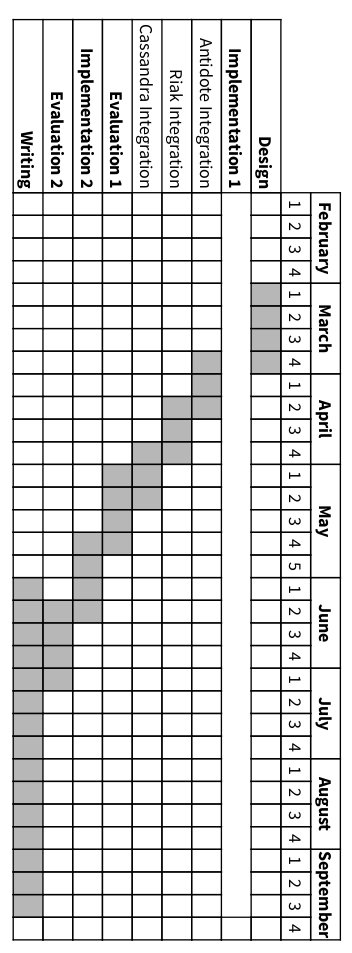
\includegraphics[scale=0.6]{files/shedule.jpg}
\caption{Schedule of activities}
\label{gant}
\end{figure}